\documentclass[11pt,a4paper]{article}

\usepackage[margin=2.3cm]{geometry}
\usepackage[T1]{fontenc}
\usepackage[utf8]{inputenc}
\usepackage{lmodern}
\usepackage{amsmath,amssymb}
\usepackage{graphicx}
\usepackage{booktabs}
\usepackage{tabularx}
\usepackage{caption}
\usepackage{xcolor}
\usepackage[round,authoryear]{natbib}
\usepackage[colorlinks=true,linkcolor=blue!50!black,urlcolor=blue!50!black,citecolor=blue!50!black]{hyperref}

\graphicspath{{../figures/}}
\captionsetup{font=small,labelfont=bf}
\newcolumntype{Y}{>{\raggedright\arraybackslash}X}

\title{\textbf{An ML Emulator of FLEXPART's Convection Scheme}\\[4pt]
\large Phase 1 of a hybrid physics--machine-learning Lagrangian dispersion model}
\author{Muhammad Waqas}
\date{November 2026}

\begin{document}
\maketitle

\begin{abstract}
FLEXPART moves particles vertically in convective clouds with the Emanuel--\v{Z}ivkovi\'{c}-Rothman
scheme. This report describes Phase~1 of a hybrid model in which FLEXPART's simple equations stay as
exact physics and only complex modules are replaced by small trained models. FLEXPART~11's convection
routines (\texttt{CONVECT}, \texttt{TLIFT}) were extracted, patched and compiled as a standalone library
that labels atmospheric columns with the scheme's redistribution matrix and new cloud-base mass flux.
Four small neural networks (a convection gate, a cloud-top classifier, a mass-conserving redistribution
network and a cloud-base mass-flux regressor; $\approx$1.9~MB in total) were trained on 82\,656 ERA5
columns of the tropical Indian Ocean (2019--2021). On the unseen year 2023 they reproduce the mean
upward mass-flux profile within 10.9\% at the worst level, conserve mass exactly, and reach a median
per-column error of 34\% in the moved air. On the tropical Atlantic, a region never seen in training,
all errors stay within 1.13 times the Indian Ocean values. The emulator is only 1.3--1.6 times faster
than the Fortran scheme on a CPU, so the case for the approach rests on accuracy and on learning
better physics in later phases, not on speed.
\end{abstract}

\section{Motivation}
FLEXPART \citep[][]{stohl2005,pisso2019,bakels2024} is a chain of physical steps: interpolation of
meteorological fields, particle release, turbulence statistics, the Langevin equation, advection,
convection, removal processes and concentration sampling. Most steps are short closed-form formulas,
which a neural network cannot improve on. A few are expensive or empirical: the convection scheme
\citep{emanuel1999,forster2007}, the turbulence statistics and wet scavenging. The overall plan
(Table~\ref{tab:phases}) replaces only those modules with trained models, keeping the particle
framework, advection and mass bookkeeping as exact physics. Convection is the first target: it is the
heaviest physics module per time step, it decides how much ocean-emitted gas (e.g.\ bromoform) is
lifted towards the tropopause, and its mapping from a column profile to a redistribution matrix is
deterministic. The approach follows the idea of learned sub-grid parameterisations in climate models
\citep{rasp2018}; ML emulators of whole dispersion-model footprints exist \citep{fillola2023,he2025},
but they bypass the physics instead of replacing single modules.

\begin{table}[h]
\centering\small
\begin{tabularx}{\textwidth}{lYl}
\toprule
Phase & Work & Status \\
\midrule
1 & Offline emulator of FLEXPART's convection scheme, trained on FLEXPART's own code & essentially complete \\
2 & Coupling into FLEXPART (TorchScript model called from Fortran via FTorch); long online runs & next \\
3 & ML turbulence and wet-scavenging modules trained on LES or observations, aiming to beat the original fits & planned \\
4 & Validation of the hybrid model against ship and aircraft observations & planned \\
\bottomrule
\end{tabularx}
\caption{Project phases.}
\label{tab:phases}
\end{table}

\section{Methods}

\subsection{FLEXPART's convection scheme as the teacher}
For each column, FLEXPART fills module arrays with temperature $T$, specific humidity $q$, saturation
humidity $q_s$ and full- and half-level pressures, and calls \texttt{CONVECT}. The scheme returns the
mass flux $f_{ij}$ (kg\,m$^{-2}$\,s$^{-1}$) from level $i$ to level $j$ and updates the cloud-base mass
flux $m_b$, which must be carried between calls: the scheme has memory. FLEXPART's \texttt{calcmatrix}
turns $f_{ij}$ into a mass matrix; dividing each row by the layer mass gives the redistribution
matrix of fractions used here,
\begin{equation}
M_{ij} = \frac{\Delta t\, f_{ij} + \delta_{ij}\left(\dfrac{\Delta p_i}{g} - \Delta t\sum_k f_{ik}\right)}{\Delta p_i / g},
\qquad \sum_j M_{ij} = 1 ,
\end{equation}
where $\Delta p_i$ is the pressure thickness of level $i$ and $\Delta t = 900$~s.

\texttt{CONVECT} and \texttt{TLIFT} (lines 990--2106 of \texttt{conv\_mod.f90}, FLEXPART~11) depend
only on FLEXPART's parameter module, so they were copied into a standalone Fortran module with the
arrays they use and a C-compatible wrapper, compiled with \texttt{gfortran}, and called from Python
through \texttt{ctypes}. One change was needed: the scheme stops the program (\texttt{ERROR STOP},
``Convection reaches top level of input data'') when convection approaches the top of the column, which
killed the Python session. The statement was replaced by a flag, and such columns are returned with
\texttt{iflag}~$=-1$ and dropped. Columns extend to 10~hPa, which made this case rare (0.1\% of
columns in a synthetic test). In tests, the scheme behaved as expected: convective columns gave
\texttt{iflag}~$=1$ with $m_b$ spinning up over successive calls (0.0029 to 0.0090~kg\,m$^{-2}$\,s$^{-1}$
in eight calls for a moist tropical column), stable columns returned the identity matrix, and all rows
summed to one.

\subsection{Data}
\textbf{ERA5} \citep{hersbach2020}: temperature and specific humidity on 32 pressure levels
(1000--10~hPa), January, April, July and October, four days per month, 00 and 12~UTC, on a 1$^\circ$
grid; 27\,552 columns per year. Tropical Indian Ocean (10$^\circ$S--10$^\circ$N, 60--100$^\circ$E):
training 2019--2021, validation 2022, test 2023. Tropical Atlantic (10$^\circ$S--10$^\circ$N,
40$^\circ$W--0$^\circ$), 2023: held-out region. Surface pressure was not downloaded; 1013~hPa is
assumed. Earlier versions (v1--v3) used synthetic soundings from four climate regimes.

\textbf{Labels.} Because of the scheme's memory, each column gets a random number (0--8) of spin-up
calls, which gives a realistic spread of the previous cloud-base mass flux $m_b^{\text{old}}$; the next
call provides the labels $M$ and $m_b^{\text{new}}$.

\textbf{Inputs} (69 features): $T$ and $q$ on 32 levels, surface pressure, CAPE, CIN and
lifting condensation level pressure from a parcel ascent, and $m_b^{\text{old}}$.

\subsection{Models}
\begin{enumerate}
\item \textbf{Gate} (MLP, $2\times128$): probability that convection is active.
\item \textbf{Cloud top} (MLP, $2\times128$, 32 classes): highest level touched by the convection. At
prediction time the \emph{cautious} cloud top is used: the smallest level $k$ with
$P(\text{top}\le k)\ge 0.95$.
\item \textbf{Redistribution network} (MLP, $3\times256$, input: features plus the one-hot cloud top
$k$; output: $32\times32$ scores $z_{ij}$). Entries above the cloud top are masked and a row-wise
softmax gives
\begin{equation}
\hat M_{ij} = \frac{\exp z_{ij}}{\sum_{l \in A_i} \exp z_{il}}\quad (j \in A_i), \qquad
A_i = \begin{cases}\{0,\dots,k\} & i \le k\\ \{i\} & i > k\end{cases}
\end{equation}
so every row is non-negative and sums to one (mass is conserved exactly) and no air goes above the
cloud top.
\item \textbf{Cloud-base mass flux} (MLP, $2\times64$, softplus output): $m_b^{\text{new}}$.
\end{enumerate}

\textbf{Loss.} The redistribution network minimises a row-weighted KL divergence,
\begin{equation}
\mathcal{L}_{\text{KL}} = \sum_i w_i \sum_j M_{ij}\ln\frac{M_{ij}}{\hat M_{ij}},\qquad
w_i = 0.8\,\frac{\Delta p_i(1-M_{ii})}{\sum_l \Delta p_l(1-M_{ll})} + 0.2\,\frac{\Delta p_i}{\sum_l \Delta p_l},
\end{equation}
which weights rows by the air FLEXPART actually moves out of them. During training the network
receives the true cloud top plus a random 0--3 levels of slack. After 60 epochs, a 10-epoch
fine-tuning stage (learning rate $10^{-4}$) adds the relative error of the upward and downward mass
fluxes $F_k$ across every level interface $k$,
\begin{equation}
\mathcal{L} = \mathcal{L}_{\text{KL}} + 0.1\left(\frac{\overline{(\hat F^{\uparrow}-F^{\uparrow})^2}}{\overline{(F^{\uparrow})^2}}
+ \frac{\overline{(\hat F^{\downarrow}-F^{\downarrow})^2}}{\overline{(F^{\downarrow})^2}}\right),
\qquad F^{\uparrow}_k = \sum_{i\le k}\sum_{j>k}\Delta p_i M_{ij}.
\end{equation}

\subsection{Validation}
On the test set: gate F1; cloud-top accuracy; mean absolute matrix error; the worst-level relative
error of the mean upward mass-flux profile; the per-column relative error of the off-diagonal part of
the matrix (the air that actually moves), $\sum_{i\neq j}|\hat M_{ij}-M_{ij}| / \sum_{i\neq j} M_{ij}$,
overall and for the 10\% of columns with the strongest convection; a particle test (1-D Wasserstein
distance between final-pressure distributions of mass-weighted particles); $R^2$ of
$m_b^{\text{new}}$; and speed per column on a CPU.

\section{Development history}
Table~\ref{tab:history} summarises the five versions. Two lessons shaped the final design. First,
averaged metrics hide structural errors: v2's matrix error was tiny ($5.7\times10^{-5}$) because most
entries are trivially near 0 or 1, yet single columns were visibly blurred
(Fig.~\ref{fig:v2v3}a): when unsure whether the cloud stops at one level or another, the network spread
air over both. The cloud-top model and masking (v3) removed this hedging and also removed the
boundary-layer flux bias. Second, a mass-flux loss switched on from the start collapsed training:
the untrained network's fluxes were thousands of times too large, and the quickest way to reduce a
\emph{relative} flux error was to move no air at all (Fig.~\ref{fig:v2v3}b). Used only as a
fine-tuning stage (v5), the same term removed the 15--20\% flux overestimate seen on ERA5 in v4.

\begin{table}[h]
\centering\small
\begin{tabular}{llcccccc}
\toprule
Version & Data & Gate F1 & Top exact & Flux err. & Off-diag. err. & $R^2(m_b)$ & Speed-up \\
\midrule
v2 & synthetic & 0.956 & -- & 10.9\% & -- & 0.964 & 2.6$\times$ \\
v3, flux loss 0.1 & synthetic & 0.961 & 0.845 & 865\% & 122\% & 0.964 & 1.5$\times$ \\
v3, no flux loss & synthetic & 0.961 & 0.845 & 4.7\% & 57\% & 0.964 & 1.6$\times$ \\
v4 & ERA5 & 0.989 & 0.791 & 28.2\% & 34\% & 0.990 & 1.3$\times$ \\
\textbf{v5} & \textbf{ERA5} & \textbf{0.989} & \textbf{0.827} & \textbf{10.9\%} & \textbf{34\%} & \textbf{0.990} & \textbf{1.4$\times$} \\
\bottomrule
\end{tabular}
\caption{Development history. Flux error: worst-level relative error of the mean upward mass flux.
Off-diagonal error: median per-column relative error of the moved air. Synthetic and ERA5 results are
not directly comparable. v1 used a simplified stand-in scheme and is omitted.}
\label{tab:history}
\end{table}

\begin{figure}[h]
\centering
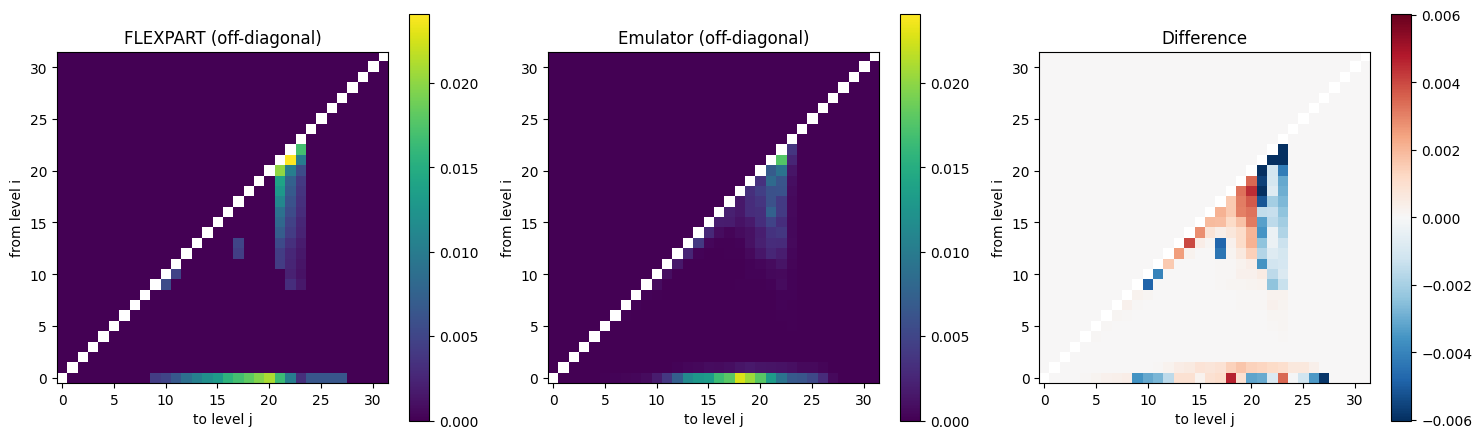
\includegraphics[width=\textwidth]{v2_synthetic_strongest_column.png}\\[-1pt]
{\small (a) v2: the emulator blurs the sharp structure of FLEXPART's matrix.}\\[6pt]
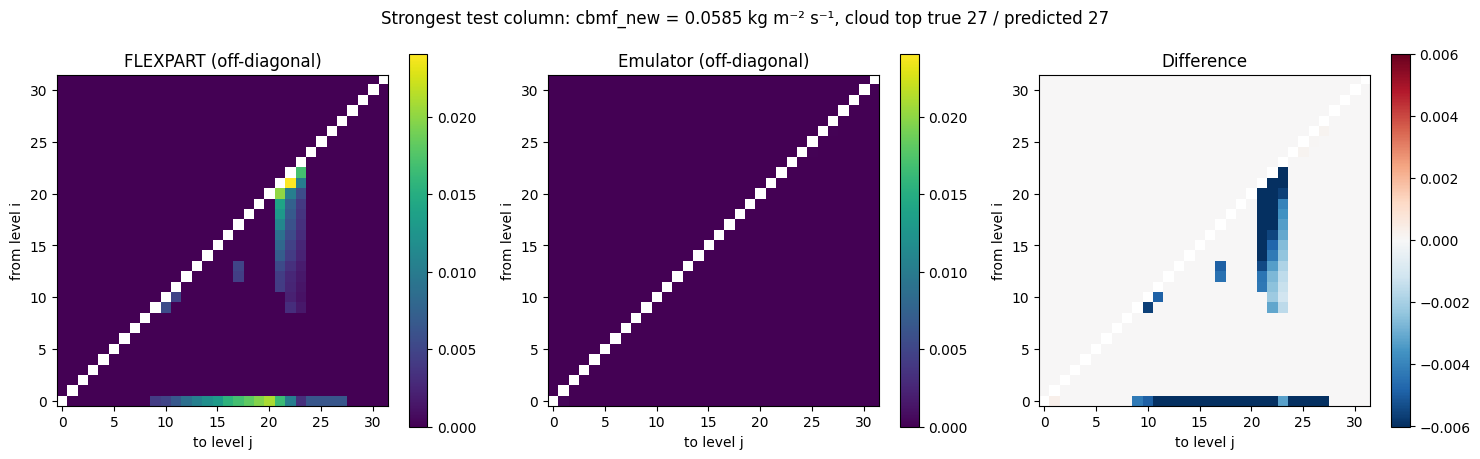
\includegraphics[width=\textwidth]{v3_fluxloss_failure_strongest_column.png}\\[-1pt]
{\small (b) v3 with a flux loss from the start: the emulator collapses to ``no air moves''.}
\caption{Off-diagonal part of the redistribution matrix for the strongest-convection test column
(FLEXPART, emulator, difference; synthetic data).}
\label{fig:v2v3}
\end{figure}

\section{Results (v5)}

\subsection{Unseen year: tropical Indian Ocean, 2023}
On 27\,552 test columns (25\,359 convective), the gate reaches F1 = 0.989 (24\,858 hits, 53 false
alarms, 501 misses). The most likely cloud top is exact in 82.7\% of convective columns and within one
level in 93.7\%; the cautious cloud top lies at or above the true one in 99.0\% of columns, at a cost
of only 0.78 extra levels on average. The mean upward mass-flux profile matches FLEXPART from the
surface to the stratosphere (Fig.~\ref{fig:v5}, top), with a worst-level error of 10.9\%. The median
per-column error of the moved air is 34\% (33\% for the strongest 10\%), the median particle
Wasserstein distance is 0.014~hPa, $R^2(m_b^{\text{new}}) = 0.990$, and every row sums to one.

The strongest test column illustrates the cautious cloud top (Fig.~\ref{fig:v5}, bottom): the most
likely cloud top was wrong (level 5 instead of 13), which in v4 had wiped out the column, but the
cautious top was exactly right, and the emulator reproduces FLEXPART's structure: the surface updraft
spread over levels 2--13 and the shallow mixing just above the diagonal.

Real ERA5 convection over the Indian Ocean differs from the synthetic soundings: the upward flux is
largest at the surface and decreases steadily with height, and much of the moved air mixes only one
to three levels upward.

\begin{figure}[h]
\centering
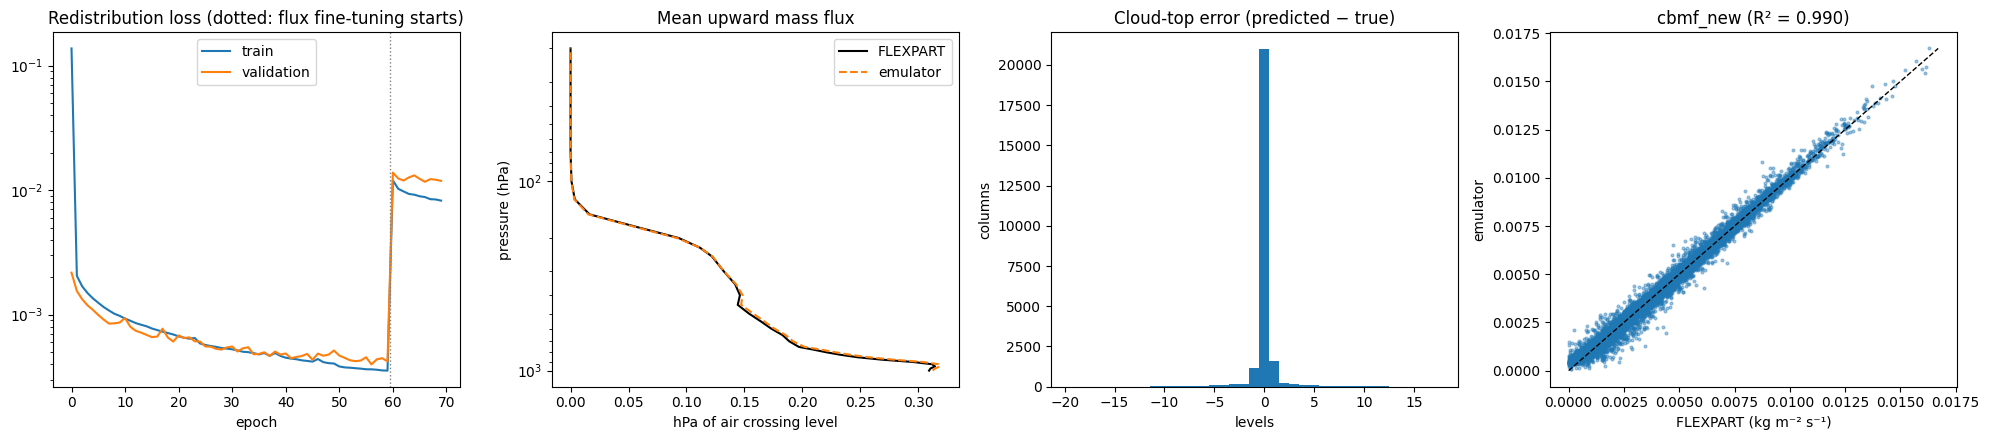
\includegraphics[width=\textwidth]{v5_era5_summary.png}\\[4pt]
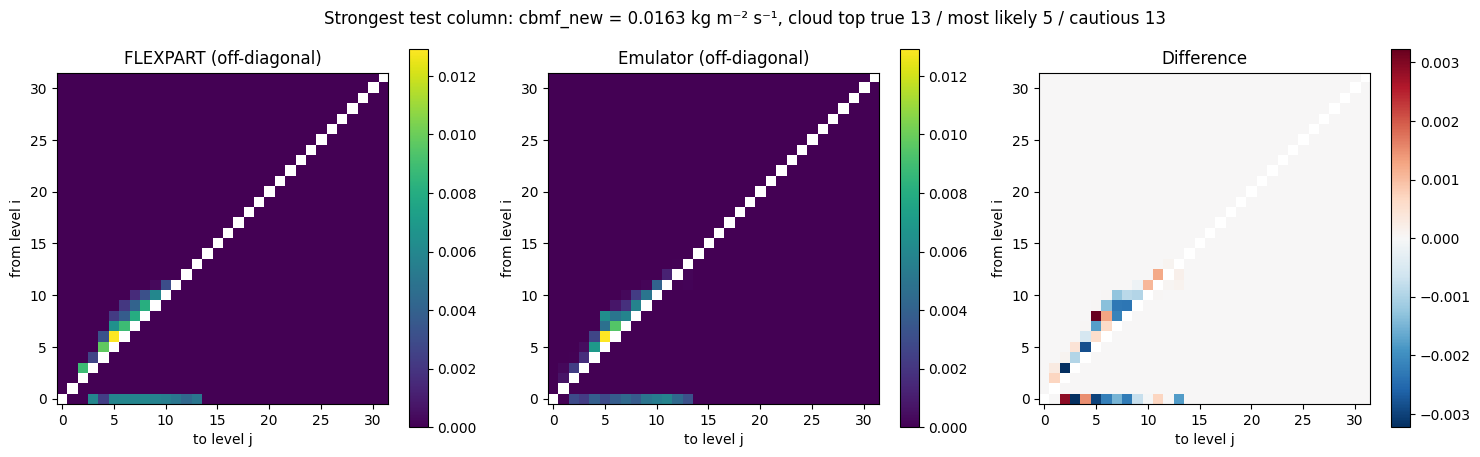
\includegraphics[width=\textwidth]{v5_era5_strongest_column.png}
\caption{v5 on the Indian Ocean test year 2023. Top: training loss (dotted line: start of flux
fine-tuning), mean upward mass flux, cloud-top error and $m_b^{\text{new}}$. Bottom: off-diagonal
matrix of the strongest test column.}
\label{fig:v5}
\end{figure}

\subsection{Unseen region: tropical Atlantic, 2023}
Table~\ref{tab:atlantic} compares the two test sets. Every error stays within 1.13 times the Indian
Ocean value, meeting the target of 1.5; the mass-flux profile is matched even better
(Fig.~\ref{fig:atl}). The off-diagonal error histogram shows a spike at exactly 1.0
(about 800 columns), where the emulator moved no air while FLEXPART did: these are columns where the
gate missed weak convection, which also appear as zeros in the $m_b^{\text{new}}$ scatter.

\begin{table}[h]
\centering\small
\begin{tabular}{lccc}
\toprule
Check & Indian Ocean 2023 & Atlantic 2023 (unseen) & Ratio \\
\midrule
Gate F1 & 0.989 & 0.976 & -- \\
Cautious top $\ge$ true top & 99.0\% & 98.5\% & -- \\
Mass flux, worst level & 10.9\% & 7.9\% & 0.73 \\
Off-diagonal error, median & 33.9\% & 37.9\% & 1.12 \\
Off-diagonal error, strongest 10\% & 33.2\% & 37.5\% & 1.13 \\
Particle test, median & 0.014 hPa & 0.013 hPa & 0.93 \\
$R^2(m_b^{\text{new}})$ & 0.990 & 0.965 & -- \\
\bottomrule
\end{tabular}
\caption{Generalisation to a region never seen in training. Convective share: 92\% (Indian Ocean
test) and 86\% (Atlantic).}
\label{tab:atlantic}
\end{table}

\begin{figure}[h]
\centering
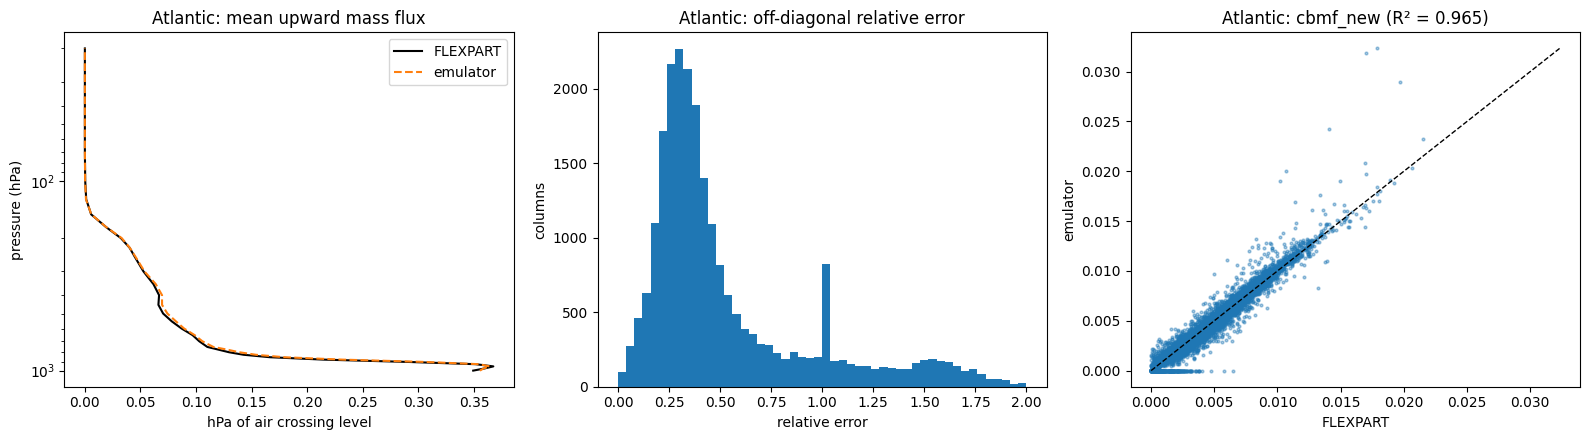
\includegraphics[width=\textwidth]{v5_atlantic_heldout_summary.png}
\caption{v5 on the tropical Atlantic 2023 (held-out region): mean upward mass flux, per-column
off-diagonal error and $m_b^{\text{new}}$.}
\label{fig:atl}
\end{figure}

\subsection{Speed}
FLEXPART's scheme takes about 50--90~$\mu$s per column in these tests (including Python call
overhead); the four-model emulator takes about 38~$\mu$s per column in batches on a CPU, a speed-up of
only 1.3--1.6. Called one column at a time inside FLEXPART, the advantage would shrink further.

\section{Discussion}
\textbf{What worked.} Extracting the real scheme made true labels cheap (about 0.2~ms per call). A
masked, row-wise softmax conserves mass exactly by construction. The cloud-top model, used cautiously,
removed the blurring and made cloud-top mistakes cheap. Weighting rows by moved air and a late
flux fine-tuning stage brought the mass-flux profile into agreement.

\textbf{What did not.} A flux loss from the start collapsed training. Speed was the weakest
argument: the Emanuel scheme is cheaper than expected.

\textbf{Limitations.} Offline only; surface pressure fixed at 1013~hPa; ERA5 pressure levels instead
of FLEXPART's model levels; a 1$^\circ$ grid and two regions; and FLEXPART's \texttt{nconvtop} lies one
level above the highest level with mass flux, which may place cloud tops slightly high.

\textbf{Next steps.} (1) Lower the gate threshold to recover weak convection; (2) add surface
pressure and model-level input; (3) Phase~2: call the TorchScript model from FLEXPART's Fortran code
via FTorch and run long simulations; (4) Phase~3: train turbulence or scavenging modules on LES or
observations, where an ML module could be more accurate than the original empirical fits.

\section*{Code and data}
Notebooks, scripts, results and figures: this repository. FLEXPART is downloaded from its official
repository at run time; ERA5 data from the Copernicus Climate Data Store.

\begin{thebibliography}{99}
\bibitem[Bakels et~al.(2024)]{bakels2024} Bakels, L., et~al. (2024). Version 11 of the Lagrangian
particle dispersion model FLEXPART. \emph{Geosci. Model Dev.}, 17.
\bibitem[Emanuel and \v{Z}ivkovi\'{c}-Rothman(1999)]{emanuel1999} Emanuel, K.~A. and
\v{Z}ivkovi\'{c}-Rothman, M. (1999). Development and evaluation of a convection scheme for use in
climate models. \emph{J. Atmos. Sci.}, 56, 1766--1782.
\bibitem[Fillola et~al.(2023)]{fillola2023} Fillola, E., et~al. (2023). A machine learning emulator for
Lagrangian particle dispersion model footprints: a case study using NAME. \emph{Geosci. Model Dev.},
16, 1997.
\bibitem[Forster et~al.(2007)]{forster2007} Forster, C., Stohl, A. and Seibert, P. (2007).
Parameterization of convective transport in a Lagrangian particle dispersion model and its evaluation.
\emph{J. Appl. Meteor. Climatol.}, 46, 403--422.
\bibitem[He et~al.(2025)]{he2025} He, T.-L., et~al. (2025). FootNet v1.0: development of a machine
learning emulator of atmospheric transport. \emph{Geosci. Model Dev.}, 18, 1661.
\bibitem[Hersbach et~al.(2020)]{hersbach2020} Hersbach, H., et~al. (2020). The ERA5 global reanalysis.
\emph{Q. J. R. Meteorol. Soc.}, 146, 1999--2049.
\bibitem[Pisso et~al.(2019)]{pisso2019} Pisso, I., et~al. (2019). The Lagrangian particle dispersion
model FLEXPART version 10.4. \emph{Geosci. Model Dev.}, 12, 4955--4997.
\bibitem[Rasp et~al.(2018)]{rasp2018} Rasp, S., Pritchard, M.~S. and Gentine, P. (2018). Deep learning
to represent subgrid processes in climate models. \emph{PNAS}, 115, 9684--9689.
\bibitem[Stohl et~al.(2005)]{stohl2005} Stohl, A., et~al. (2005). Technical note: The Lagrangian
particle dispersion model FLEXPART version 6.2. \emph{Atmos. Chem. Phys.}, 5, 2461--2474.
\end{thebibliography}

\end{document}
